\documentclass[letterpaper]{article} % DO NOT CHANGE THIS
\usepackage[submission]{aaai2027}  % DO NOT CHANGE THIS
\usepackage[hyphens]{url}  % DO NOT CHANGE THIS
\usepackage{graphicx} % DO NOT CHANGE THIS
\urlstyle{rm} % DO NOT CHANGE THIS
\def\UrlFont{\rm}  % DO NOT CHANGE THIS
\usepackage{natbib}  % DO NOT CHANGE THIS AND DO NOT ADD ANY OPTIONS TO IT
\usepackage{caption} % DO NOT CHANGE THIS AND DO NOT ADD ANY OPTIONS TO IT
\frenchspacing  % DO NOT CHANGE THIS
\usepackage{booktabs}
\usepackage{amsmath}
\usepackage{amssymb}
\usepackage{algorithm}
\usepackage{algorithmic}

\pdfinfo{
/TemplateVersion (2027.1)
}

\setcounter{secnumdepth}{0}

\title{LLM-Governed Action Constraints for Fault-Tolerant\\
Reinforcement Learning}

\author{
    Anonymous Submission
}
\affiliations{
    Anonymous Submission
}

\begin{document}

\maketitle

% ============================ ABSTRACT ============================
\begin{abstract}
Deep reinforcement learning (DRL) can match or beat heuristics on average, but in
stochastic environments its learned policies are often \emph{unreliable}: under
the intrinsic nondeterminism of a high-fidelity simulator, identically configured
runs sometimes converge to good policies and sometimes fail catastrophically.
Existing safe-RL methods mostly reshape the reward or add static constraints,
which we show is insufficient. We propose to treat a large language model (LLM)
not as a policy generator but as an \emph{adaptive governance module} that
improves the dependability of an off-the-shelf DRL agent: after each episode a
locally hosted LLM reads the run's KPIs and emits human-readable safety rules,
which a deterministic layer compiles into per-step action masks. We instantiate
this on a demanding, resource-critical case study---urgent-lot scheduling in a
semiconductor digital twin built from real factory data---where pure DRL fails in
60\% of independent runs ($N{=}20$ seeds). Across 20 seeds our method cuts the
catastrophic-failure rate from 60\% to 15\% and mean cycle time by 625\,s
($p{<}0.01$), with the benefit holding across conflict regimes. A controlled
ablation that removes one design axis at a time identifies \emph{why} it works:
replacing the hard mask with equivalent reward shaping is \emph{worse} than
ungoverned DRL ($p{<}0.001$); unconditioned masking fails 45 percentage points
more often ($p{<}0.05$); and a fixed, non-adaptive rule matches the average yet
leaves the catastrophic tail intact. The gain comes specifically from
\emph{hard, contextual, and adaptive} action constraints---properties an LLM
supplies zero-shot, locally, and auditably. We argue this reframes LLM-over-DRL
governance as a general fault-tolerance mechanism for dependable RL.
\end{abstract}

% ============================ 1. INTRODUCTION ============================
\section{Introduction}

Semiconductor manufacturing lines are stochastic, non-stationary scheduling
environments. A single dispatching decision reshapes the work-in-process
distribution and influences cycle time hours later, so an action at time $t$
carries long-horizon consequences that are hard to attribute and harder to
optimize with fixed heuristics \citep{moyne2017,hu2019}. A now-standard response
couples a \emph{digital twin}---a high-fidelity discrete-event simulation of the
line---with deep reinforcement learning (DRL), learning a dispatching policy
directly from the simulated environment \citep{waschneck2018,lee2025}.
Figure~\ref{fig:drlbase} illustrates this baseline coupling: the digital twin
supplies shop-floor state and receives dispatching actions, while a value-based
agent learns via experience replay.

\begin{figure}[t]
  \centering
  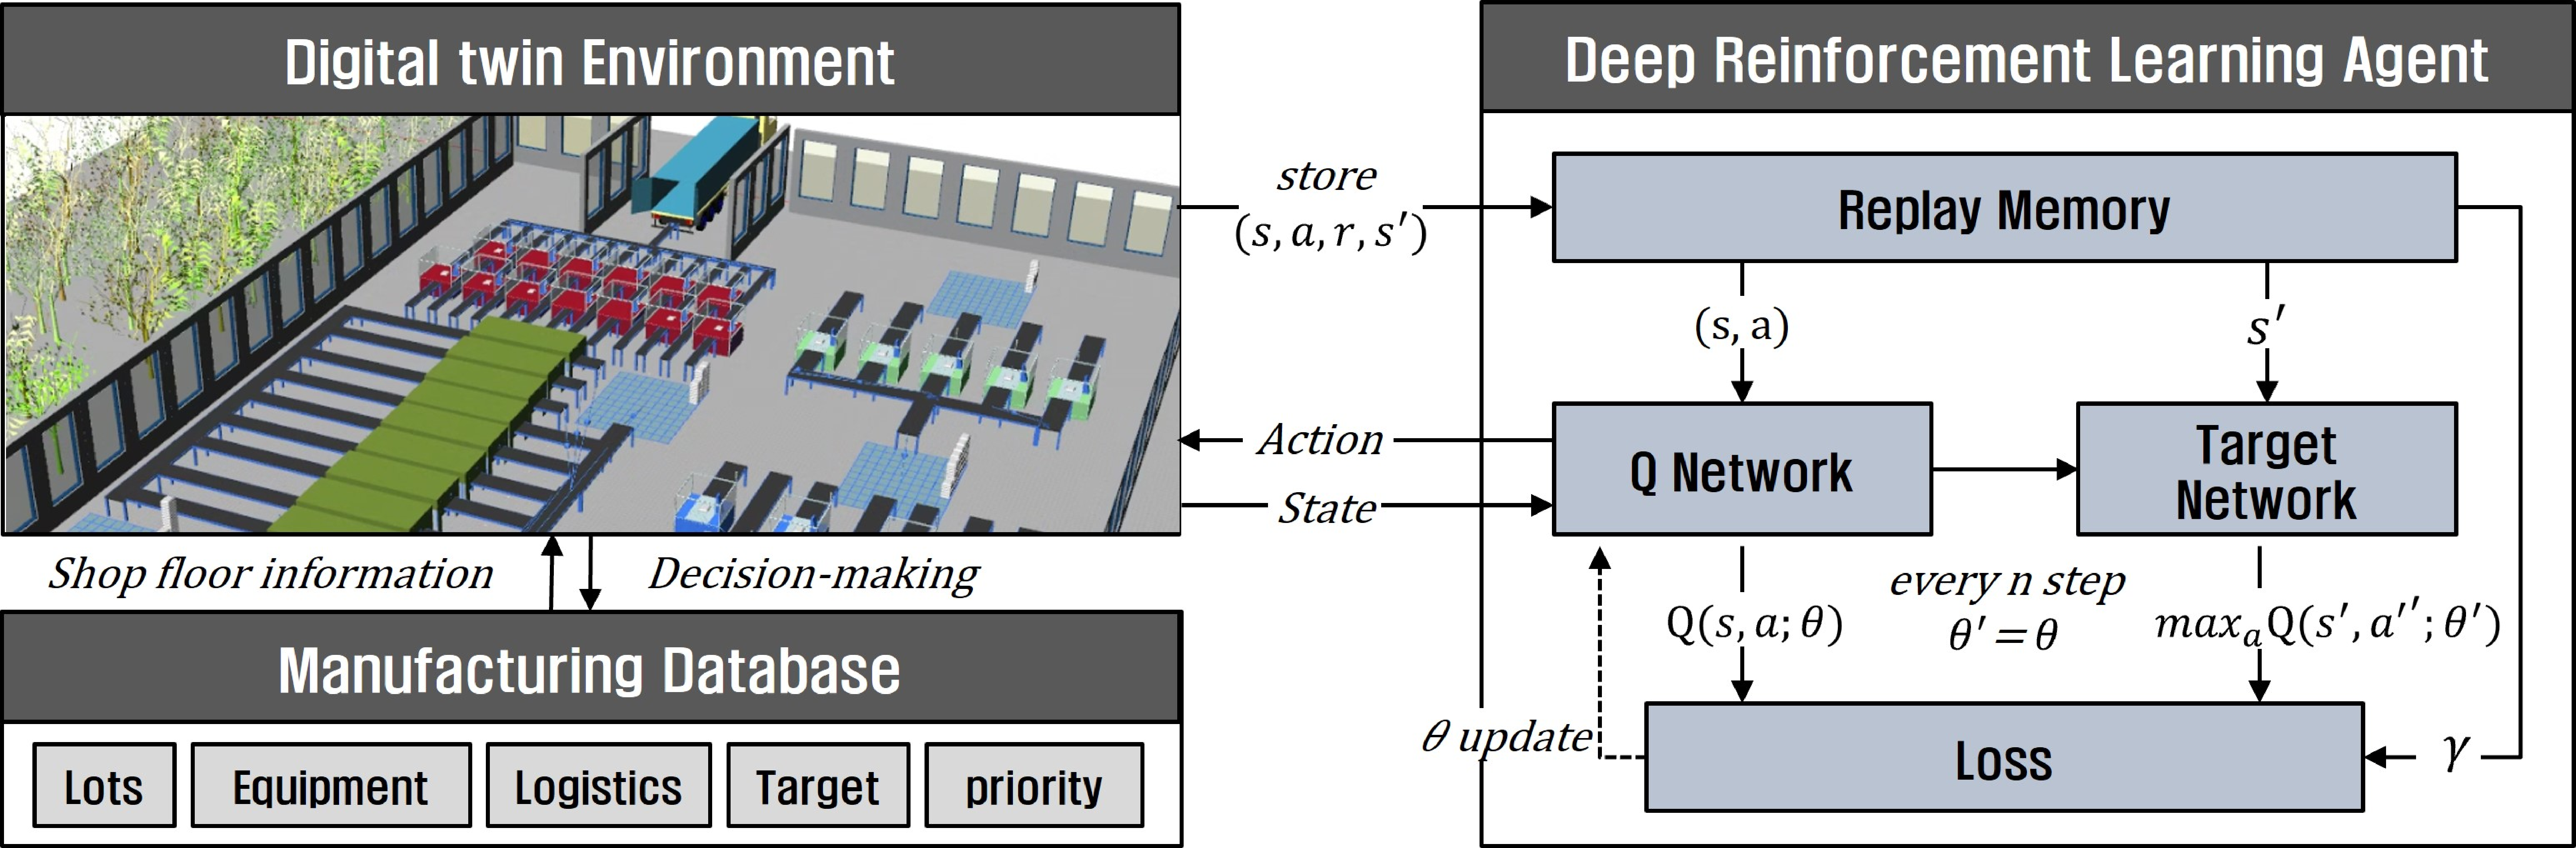
\includegraphics[width=0.92\columnwidth]{Figures/fig_drlbaseline.pdf}
  \caption{Baseline DRL scheduling loop. The digital twin acts as the training
  environment; the agent observes shop-floor state $s$, selects a dispatching
  action $a$, receives reward $r$, and updates its Q-network. This coupling is
  effective on average but, as we show, unreliable from run to run.}
  \label{fig:drlbase}
\end{figure}

Despite encouraging average-case results, deploying DRL in cost- and
yield-critical manufacturing surfaces a problem the literature rarely
quantifies: the learned policy is \emph{not reliable from run to run}. Because
the digital twin is internally nondeterministic, identically configured training
runs can converge to a high-quality policy in one run and fail catastrophically
in another. This fragility is most acute when urgent-lot conflicts are frequent:
a small cohort of high-priority lots must traverse the line quickly, but when
they are numerous enough to create genuine contention at the bottleneck, the
reward signal for urgent handling becomes noisy and convergence becomes a matter
of chance. In dependability terms the scheduler exhibits an \emph{intermittent
fault}: under nominally identical conditions it occasionally produces a failed
schedule. The relevant question is therefore not ``how do we make DRL faster on
average?'' but a question of \emph{fault tolerance}---how do we keep an
unobservable, uncontrollable source of nondeterminism from manifesting as a
catastrophic policy? Reward shaping and static safety constraints, the standard
safe-RL levers, do not target this intermittent-failure behavior directly, and
we show they are insufficient here.

The stakes of this unreliability are high in a resource-critical fab. Many lots
carry \emph{quality-time} (Q-time) constraints---a maximum interval between
consecutive process steps, beyond which the lot must be scrapped or reworked to
preserve yield \citep{kim2018qtime}---and these time-critical lots are exactly
the ones a scheduler must expedite. When an unreliable policy lets their cycle
time blow out, Q-time windows are breached and the energy, ultrapure water, and
materials embodied in those lots are wasted \citep{boyd2012,gutowski2009}. A
catastrophic schedule is therefore not a slow average but an occasional,
irreversible loss---which is precisely why removing the failure \emph{tail},
rather than shaving the mean, is what matters here.

One remedy is to add an external governor that steers the agent toward
correct urgent-lot handling. Large language models (LLMs) are attractive
candidates: they encode domain knowledge in natural language and can emit
human-readable rules without task-specific training. Prior work has used LLMs to
decompose goals \citep{du2023}, ground policies in interactive environments
\citep{carta2023}, and translate instructions into code \citep{liang2023}.
However, simply showing that ``LLM + DRL'' improves a metric leaves the central
scientific question unanswered: \emph{what about the design actually produces the
gain?} Is it the LLM's adaptive reasoning, the act of constraining the action
space, the frequency of updates, or merely the injection of any external signal?
Without disentangling these factors, such systems are difficult to trust,
reproduce, or transfer.

This paper answers that question through a controlled study. We adopt a
three-layer hierarchical RL (HRL) framework---an LLM strategist (L2) that emits
episodic rules, a deterministic safety layer (L1) that compiles them into action
masks, and a Rainbow DQN tactical agent (L0)---and then systematically ablate
each design dimension while holding the reward function fixed. Our experiments
use $N{=}20$ independent seeds, a substantially larger reliability sample than is
typical in this literature, and report failure-rate distributions rather than
single-run means \citep{henderson2018,agarwal2021}. We study semiconductor
scheduling as a demanding, resource-critical testbed, but the phenomenon we
target---catastrophic policy failure under environment nondeterminism---and the
governance remedy we propose are not specific to it (Discussion).

Our findings stand out along three design axes. First, the full method reduces
the catastrophic-failure rate from 60\% to 15\% and mean cycle time by 625\,s
relative to pure DRL ($p{<}0.01$). Second, replacing the \emph{hard} action mask
with an equivalent \emph{reward-shaping} term makes performance \emph{worse than
ungoverned DRL} ($p{<}0.001$): the value lies in pruning unsafe actions, not in
nudging the reward. Third, an \emph{unconditioned} random mask---constraints
applied without regard to context---fails 45 percentage points more often than
our method ($p{<}0.05$), showing that \emph{when} the constraint fires is what
matters, not merely that one exists. A fourth comparison against a fixed,
non-adaptive rule shows it can match our \emph{average} cycle time yet still
fails in 60\% of runs, confirming that adaptive revision is needed to remove the
tail. Together these isolate the operative ingredient: \emph{hard, contextual,
and adaptive} action constraints.

\noindent Our contributions are:
\begin{itemize}
\setlength\itemsep{0.15em}
\item \textbf{LLM-as-governance for fault-tolerant RL.} We introduce a
hierarchical framework that uses an LLM not as a policy generator but as an
adaptive governance module, tolerating the intermittent fault of simulator
nondeterminism by hardening an off-the-shelf DRL agent with hard, KPI-conditioned
action constraints.
\item \textbf{A mechanism, not a black box.} A controlled, single-axis ablation
identifies three orthogonal properties---\emph{hard}, \emph{contextual}, and
\emph{adaptive}---as jointly responsible for the gain, separating what matters
from reward shaping, unconditioned masking, and fixed rules.
\item \textbf{Failure-rate as the evaluation criterion.} At scale ($N{=}20$
seeds) we characterize DRL's catastrophic-failure distribution and adopt
failure-rate reduction, rather than average performance, as the metric for
safety-critical RL---cutting failures from 60\% to 15\% ($p{<}0.01$) without
sacrificing throughput, consistently across conflict regimes.
\item \textbf{A resource-critical case study.} We validate the approach on
urgent-lot scheduling in a semiconductor digital twin built from real factory
data, and discuss why the same recipe transfers to other domains where rare,
costly events make reliability matter more than the mean.
\end{itemize}

% ============================ 2. RELATED WORK ============================
\section{Related Work}
\label{sec:related}

\paragraph{DRL and digital twins for scheduling.}
RL has been applied to semiconductor dispatching as an alternative to static
rule-based policies, which struggle with the long-horizon, re-entrant nature of
these lines \citep{waschneck2018,hu2019}. A common pattern pairs a discrete-event
digital twin with a value-based agent that selects among dispatching rules
\citep{lee2025}. We adopt Rainbow DQN \citep{hessel2018} for the tactical layer.
This literature overwhelmingly reports \emph{mean} performance over a few runs
and seldom analyzes \emph{reliability}---the distribution of outcomes across
independent trainings---which is exactly the property that matters when a single
bad schedule incurs large, yield-critical losses---the concern of
\emph{dependable} RL. We foreground this distributional view with $N{=}20$ seeds.

\paragraph{Sparse rewards and external steering.}
When the events that should be rewarded are rare, the agent receives little
signal and may settle into a local optimum that ignores them \citep{pathak2017}.
The classical responses are reward shaping \citep{ng1999}, which augments the
reward but creates a non-stationary, distorted learning target, and intrinsic
motivation \citep{pathak2017}, which does not guarantee \emph{which} rare
behaviors are learned. We instead constrain the action space through an external
governor, leaving the reward intact---a form of safe RL via action masking
\citep{garcia2015}. Our ablation study directly contrasts these alternatives and
shows that the action-constraint route is decisive.

\paragraph{LLMs guiding reinforcement learning.}
LLMs have been used to inject high-level knowledge into RL: decomposing
long-horizon goals \citep{du2023}, grounding policies via online RL
\citep{carta2023}, and translating instructions into executable code
\citep{liang2023}. A complementary line encodes safety as formal constraints,
e.g., translating instructions into temporal logic to prune unsafe actions
\citep{hasanbeig2020}. Our framework differs in two ways. First, governance is
\emph{continuous and KPI-driven}: the LLM re-evaluates the line state every
episode and revises its rules, rather than providing static initial guidance.
Second, it is \emph{frequency-decoupled}: the LLM operates at the episode
timescale while a lightweight safety agent enforces rules at the millisecond
dispatch timescale, an arrangement aligned with hierarchical RL in which a
high-level manager sets goals for a low-level worker \citep{vezhnevets2017}.
Critically, unlike prior work that reports only that LLM guidance helps, we
\emph{ablate} the contribution of hardness, context, and adaptivity to identify
which is responsible for the gain.

% ============================ 3. METHOD ============================
\section{Three-Layer Governance Architecture}
\label{sec:arch}

\begin{figure}[t]
    \centering
    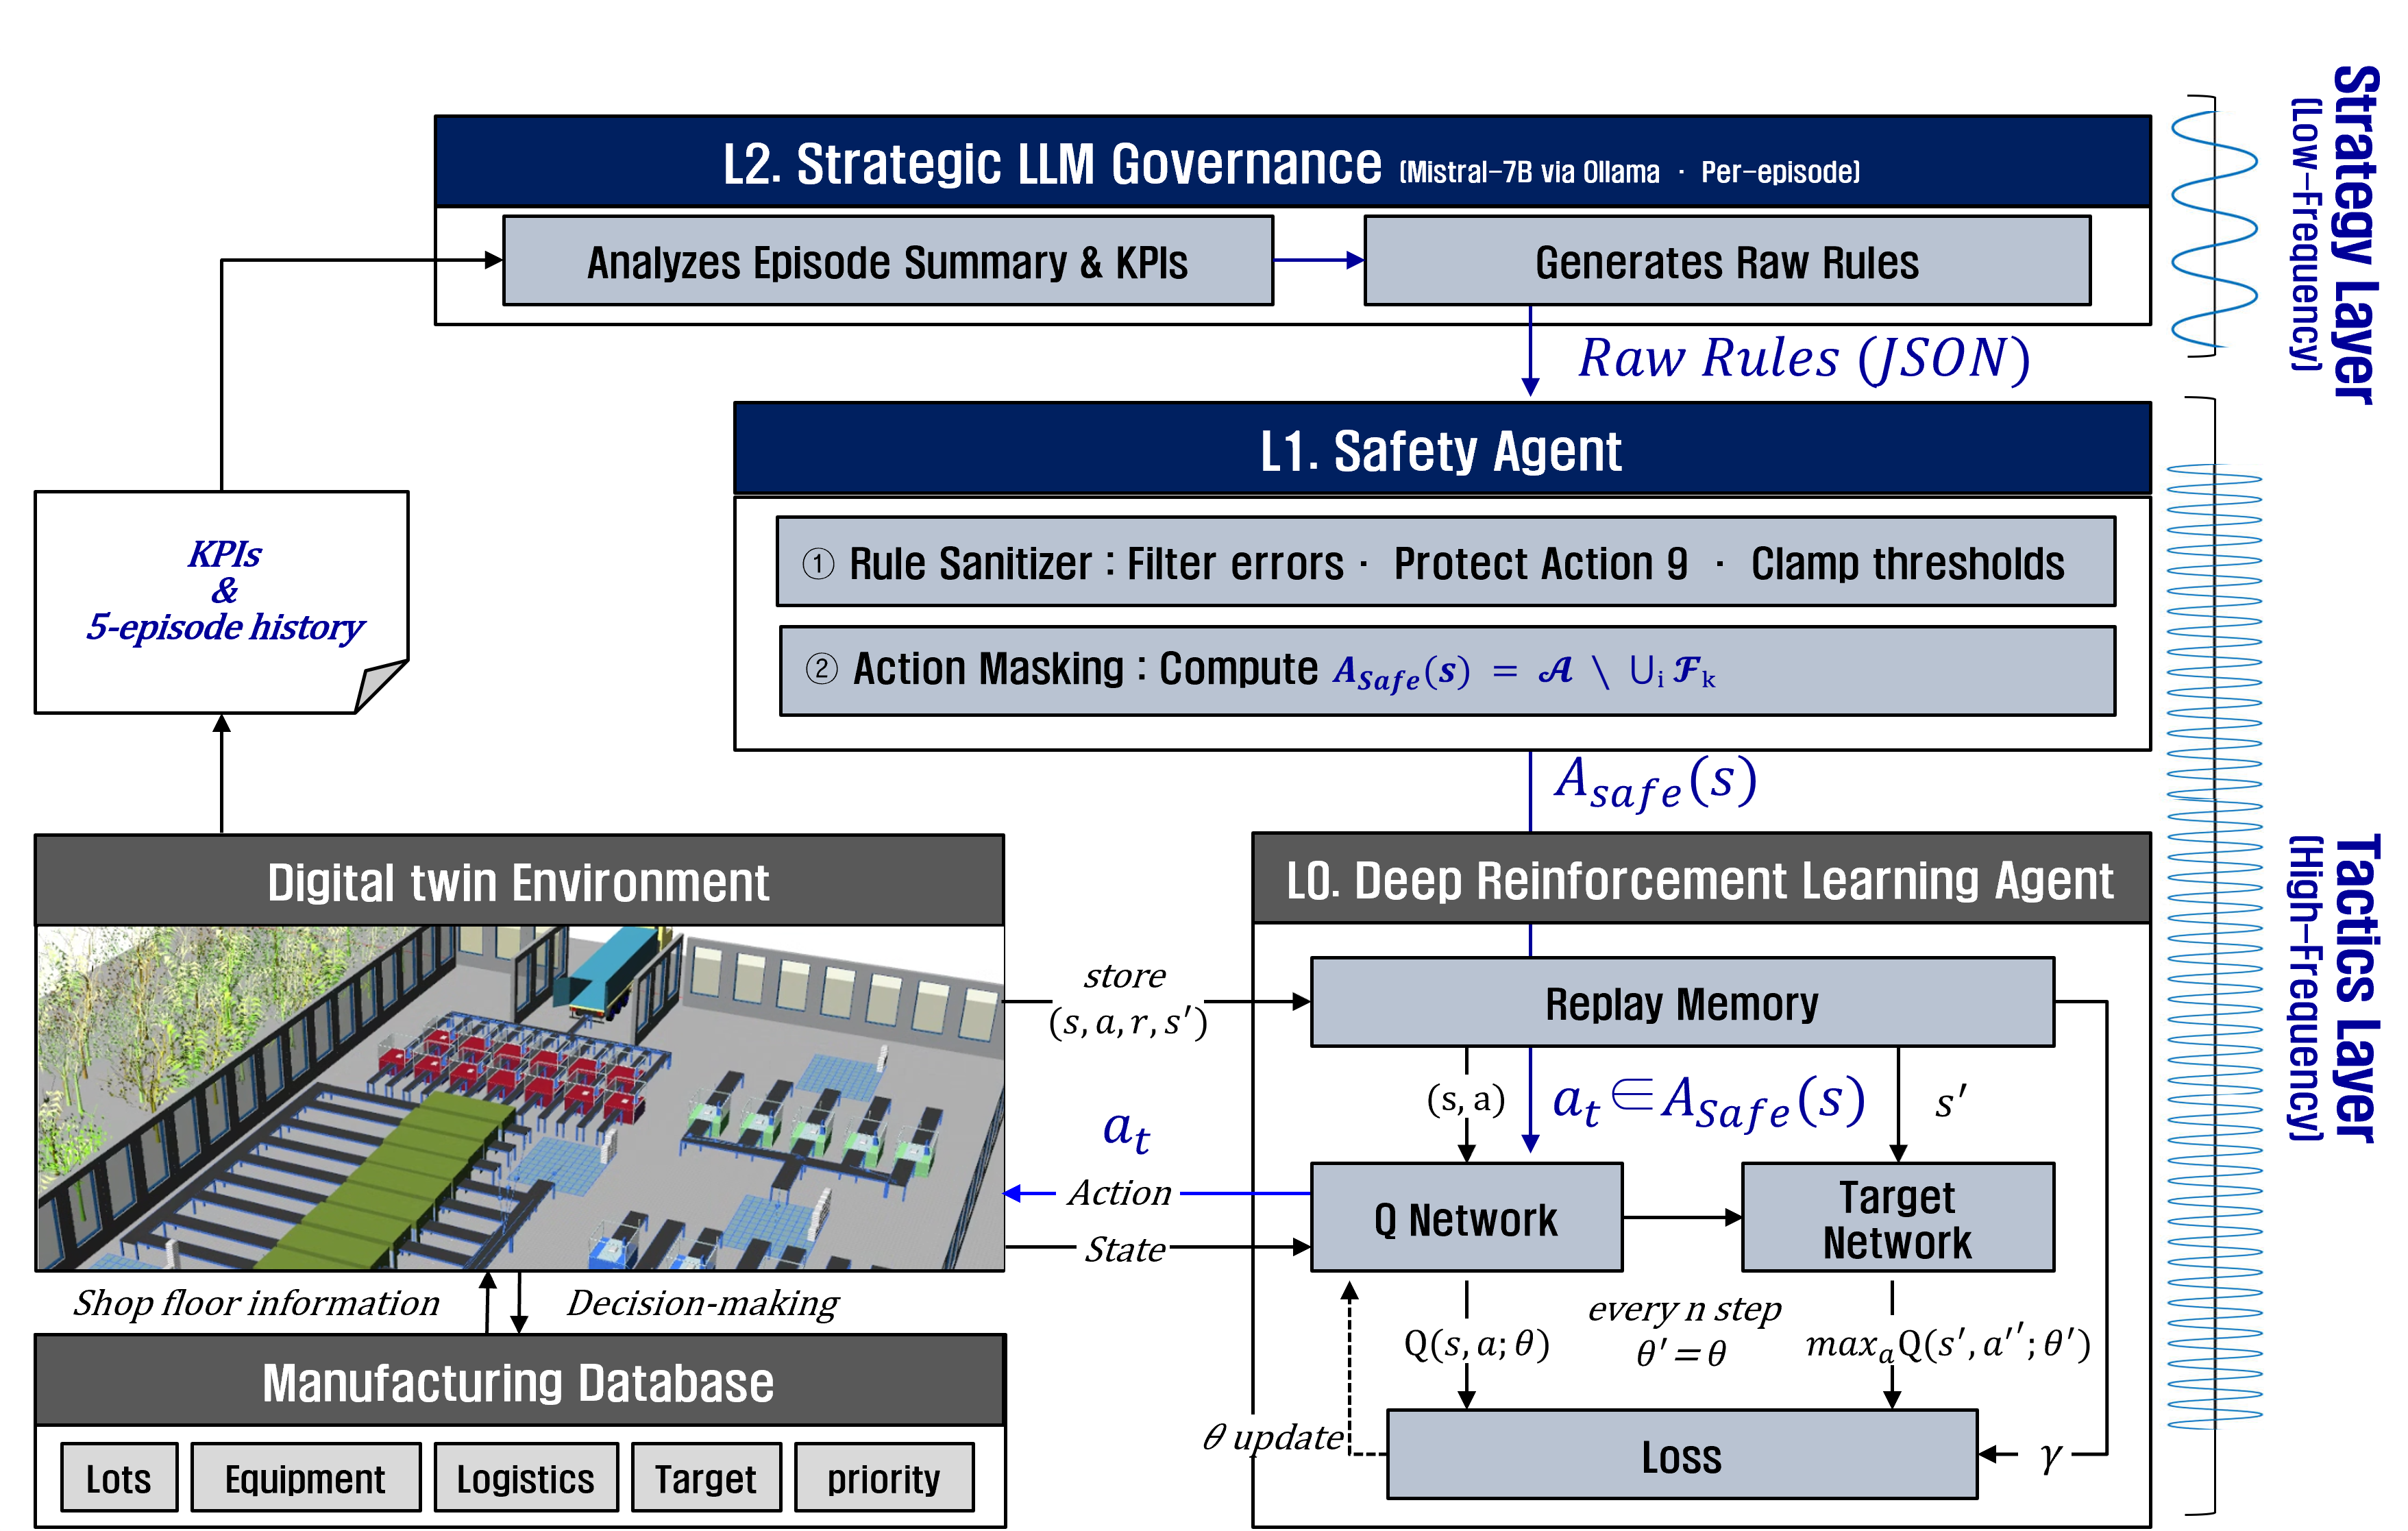
\includegraphics[width=0.96\columnwidth]{Figures/fig_architecture.png}
    \caption{Three-layer governance architecture. L2 (a locally hosted LLM)
    generates episodic safety rules from KPIs; L1 (Safety Agent) validates them
    through a built-in sanitizer and enforces per-step action masks
    (Eq.~\ref{eq:mask}); L0 (Rainbow DQN) selects the highest-value permitted
    action (Eq.~\ref{eq:constrained}). A hard-constraint floor prevents
    governance from sacrificing production attainment.}
    \label{fig:arch}
\end{figure}

Figure~\ref{fig:arch} summarizes the framework, which separates
\emph{strategy} from \emph{tactics} across three layers. Three principles
distinguish it from prior LLM-guided RL. \textbf{(i) Frequency decoupling}: the
LLM reasons once per episode while a deterministic agent enforces the rules at
every millisecond-scale step, resolving the tension between an LLM's knowledge and
the latency budget of real-time control. \textbf{(ii) Governance by action
constraint, not reward}: the LLM \emph{prunes} unsafe actions (Eq.~\ref{eq:mask})
and leaves the reward untouched, avoiding the non-stationary target reward shaping
introduces---a distinction our ablation shows is decisive. \textbf{(iii)
Safe-by-construction}: a deterministic sanitizer and a hard production floor sit
between the imperfect model and the control loop, so an erroneous rule can neither
violate safety nor sacrifice throughput, and each rule carries an auditable
natural-language rationale. We detail the layers below.

\paragraph{L2 -- Strategic governance (local LLM).}
After each training episode, a locally hosted LLM receives the episode's
aggregated KPIs (urgent-lot count and production shortage percentage) plus a
five-episode rolling history, and is prompted to (i) analyze the performance
trend, (ii) diagnose the dominant bottleneck, and (iii) emit zero or more safety
rules, each a tuple of (metric, operator, threshold, forbidden actions). The LLM
returns a structured JSON response with a rationale for every rule, and is
invoked once per episode under the frequency-decoupled design above.

\paragraph{L1 -- Safety enforcement.}
A lightweight Safety Agent receives the rule set
$\mathcal{R}=\{r_1,\dots,r_K\}$ and enforces it at every step. A built-in
sanitizer first validates each rule, discarding logically inverted predicates,
protecting the urgent-lot action from suppression, and clamping thresholds to the
per-step scale. Each validated rule $r_k=(m_k,\odot_k,\theta_k,\mathcal{F}_k)$
specifies a metric $m_k$, an operator $\odot_k\in\{>,\geq,<,\leq\}$, a threshold
$\theta_k$, and a forbidden action set $\mathcal{F}_k\subseteq\mathcal{A}$. The
\emph{safe action set} at state $s$ is
\begin{equation}
  A_{\text{safe}}(s)=\mathcal{A}\setminus
  \bigcup_{k:\,m_k(s)\,\odot_k\,\theta_k}\mathcal{F}_k,
  \label{eq:mask}
\end{equation}
and L0 selects
\begin{equation}
  a^{*}=\arg\max_{a\in A_{\text{safe}}(s)} Q(s,a;\theta).
  \label{eq:constrained}
\end{equation}
If $A_{\text{safe}}(s)=\emptyset$, a fallback reverts to the unconstrained greedy
action, preventing deadlock. The Safety Agent is deterministic and auditable.

\paragraph{L0 -- Tactical agent (Rainbow DQN).}
A Rainbow DQN agent \citep{hessel2018} operates within $A_{\text{safe}}$. It
observes a 21-dimensional state (normalized time, per-family buffer occupancy,
per-device production shortage, lead-time risk statistics, and urgent-lot counts
at the critical stage) and selects one of ten dispatching actions: nine
production-dispatching actions encoding sorting criteria and equipment
allocation, plus a single \emph{urgent-lot action} that grants highest priority
to urgent lots---the sole mechanism able to advance them ahead of ordinary queue
order. The reward decomposes as
\begin{equation}
  R(s,a)=R_{\text{prod}}(s,a)+R_{\text{urgent}}(s,a)+R_{\text{penalty}}(s,a),
  \label{eq:reward}
\end{equation}
where $R_{\text{prod}}$ captures production attainment, $R_{\text{urgent}}$
rewards urgent-lot cycle-time reductions, and $R_{\text{penalty}}$ penalizes
priority violations. Because urgent lots are at most 7.7\% of all lots,
$R_{\text{urgent}}$ is intermittent, creating the sparse-signal condition we
study.

\paragraph{Hard constraint floor.}
A hard constraint within L1 clears all active rules whenever production
attainment falls below an 85\% floor, ensuring governance never trades away the
primary production objective. Together with the sanitizer, this makes an
imperfect language model safe to deploy in the control loop.

\paragraph{The governance loop.}
Algorithm~\ref{alg:governance} ties the three layers together. Within an episode,
L1 masks and L0 acts at every dispatch step (the fast inner loop); once per
episode, L2 reads the updated KPI history and emits a revised, sanitized rule set
(the slow outer loop). The agent itself is a standard Rainbow DQN: governance is a
wrapper around an off-the-shelf learner, not a new training algorithm, which is
what makes it portable to other DRL setups.

\begin{algorithm}[t]
\caption{LLM-governed training episode}
\label{alg:governance}
\textbf{Input}: agent $Q_\theta$, active rules $\mathcal{R}$, KPI history $\mathcal{H}$\\
\textbf{Output}: updated $Q_\theta$, revised rules $\mathcal{R}$
\begin{algorithmic}[1]
\FOR{each dispatch step with state $s$}
  \STATE $A_{\text{safe}} \gets \mathcal{A}\setminus\bigcup_{k:\,m_k(s)\,\odot_k\,\theta_k}\mathcal{F}_k$ \COMMENT{L1 mask (Eq.~\ref{eq:mask})}
  \IF{$A_{\text{safe}}=\varnothing$}
     \STATE $A_{\text{safe}}\gets\mathcal{A}$ \COMMENT{deadlock fallback}
  \ENDIF
  \STATE $a\gets\arg\max_{a\in A_{\text{safe}}}Q_\theta(s,a)$; execute; store transition
  \IF{production attainment $<85\%$}
     \STATE $\mathcal{R}\gets\varnothing$ \COMMENT{hard production floor}
  \ENDIF
  \STATE update $Q_\theta$ from replay buffer
\ENDFOR
\STATE append episode KPIs to $\mathcal{H}$
\STATE $\mathcal{R}_{\text{raw}}\gets\textsc{LLM}(\mathcal{H})$ \COMMENT{L2: reason $\rightarrow$ JSON rules}
\STATE $\mathcal{R}\gets\textsc{Sanitize}(\mathcal{R}_{\text{raw}})$ \COMMENT{validate; protect urgent action}
\STATE \textbf{return} $Q_\theta,\mathcal{R}$
\end{algorithmic}
\end{algorithm}

% ============================ 4. EXPERIMENTAL SETUP ============================
\section{Experimental Setup}
\label{sec:setup}

\paragraph{Digital twin and local LLM.}
We use a Siemens Tecnomatix Plant Simulation model of a semiconductor line with
six sequential processes and heterogeneous equipment at the critical stage,
constructed from real factory data---measured lot-arrival distributions,
processing times, and routing constraints---and validated against observed
throughput and cycle-time statistics \citep{siemens2023tecnomatix}. A
research-environment policy prohibits sending production data to external
services, so we deploy Mistral-7B \citep{jiang2023} locally via Ollama as the L2
governor; the framework is model-agnostic.

\paragraph{Urgent-lot scenario and quality-time constraints.}
A small cohort of \emph{urgent} lots is injected at the line entrance and must
complete as quickly as possible. In the source facility from which our digital
twin is calibrated, such lots arise from customer samples, engineering-evaluation
lots, and expedited orders; the most consequential are those under
\emph{quality-time} (Q-time) constraints, where waiting longer than the allowed
interval between consecutive process steps forces a lot to be scrapped or
reworked \citep{kim2018qtime}---so delay does not merely slow it down but
destroys it, wasting the resources already invested. Exact urgent-lot proportions
are site-specific and commercially sensitive; we adopt a representative
$\approx$7.7\% (20 of 258 lots), within the range observed at the source
facility, and, so that our conclusions do not hinge on this single value, sweep
the ratio across regimes (Figure~\ref{fig:sweep}). At this density urgent lots create frequent bottleneck
conflicts: the urgent-handling signal is noisy relative to the throughput reward,
and DRL alone begins to fail catastrophically.

\paragraph{Metrics and failure definition.}
Our primary metric is the \emph{Urgent-Lot Cycle Time} (CT): the average
end-to-end residence time of urgent lots (lower is better). We monitor the
\emph{Target Meet Rate} (production attainment) as a constraint. Because outcomes
are distributional, we define a catastrophic-failure indicator
\begin{equation}
  F_i=\mathbf{1}\!\left[\overline{\mathrm{CT}}_i>\tau\right],\qquad
  \tau=3{,}500\,\text{s},
  \label{eq:failure}
\end{equation}
where $\overline{\mathrm{CT}}_i$ is the mean evaluation CT of run $i$. The
threshold is not an artifact of selection: pooled evaluation CT is sharply
bimodal---a success cluster near 2{,}800\,s and a failure cluster above
4{,}000\,s---and $\tau=3{,}500$\,s sits in the natural gap, with any
$\tau\in[3{,}500,4{,}000]$\,s yielding the same ordering of conditions. The
empirical failure rate is
$\hat{\rho}=\frac{1}{N}\sum_i F_i$, and the quantity of interest is the
failure-rate reduction $\Delta\rho=\hat{\rho}_{\text{DRL}}-\hat{\rho}_{\text{ours}}$.

\begin{figure}[t]
  \centering
  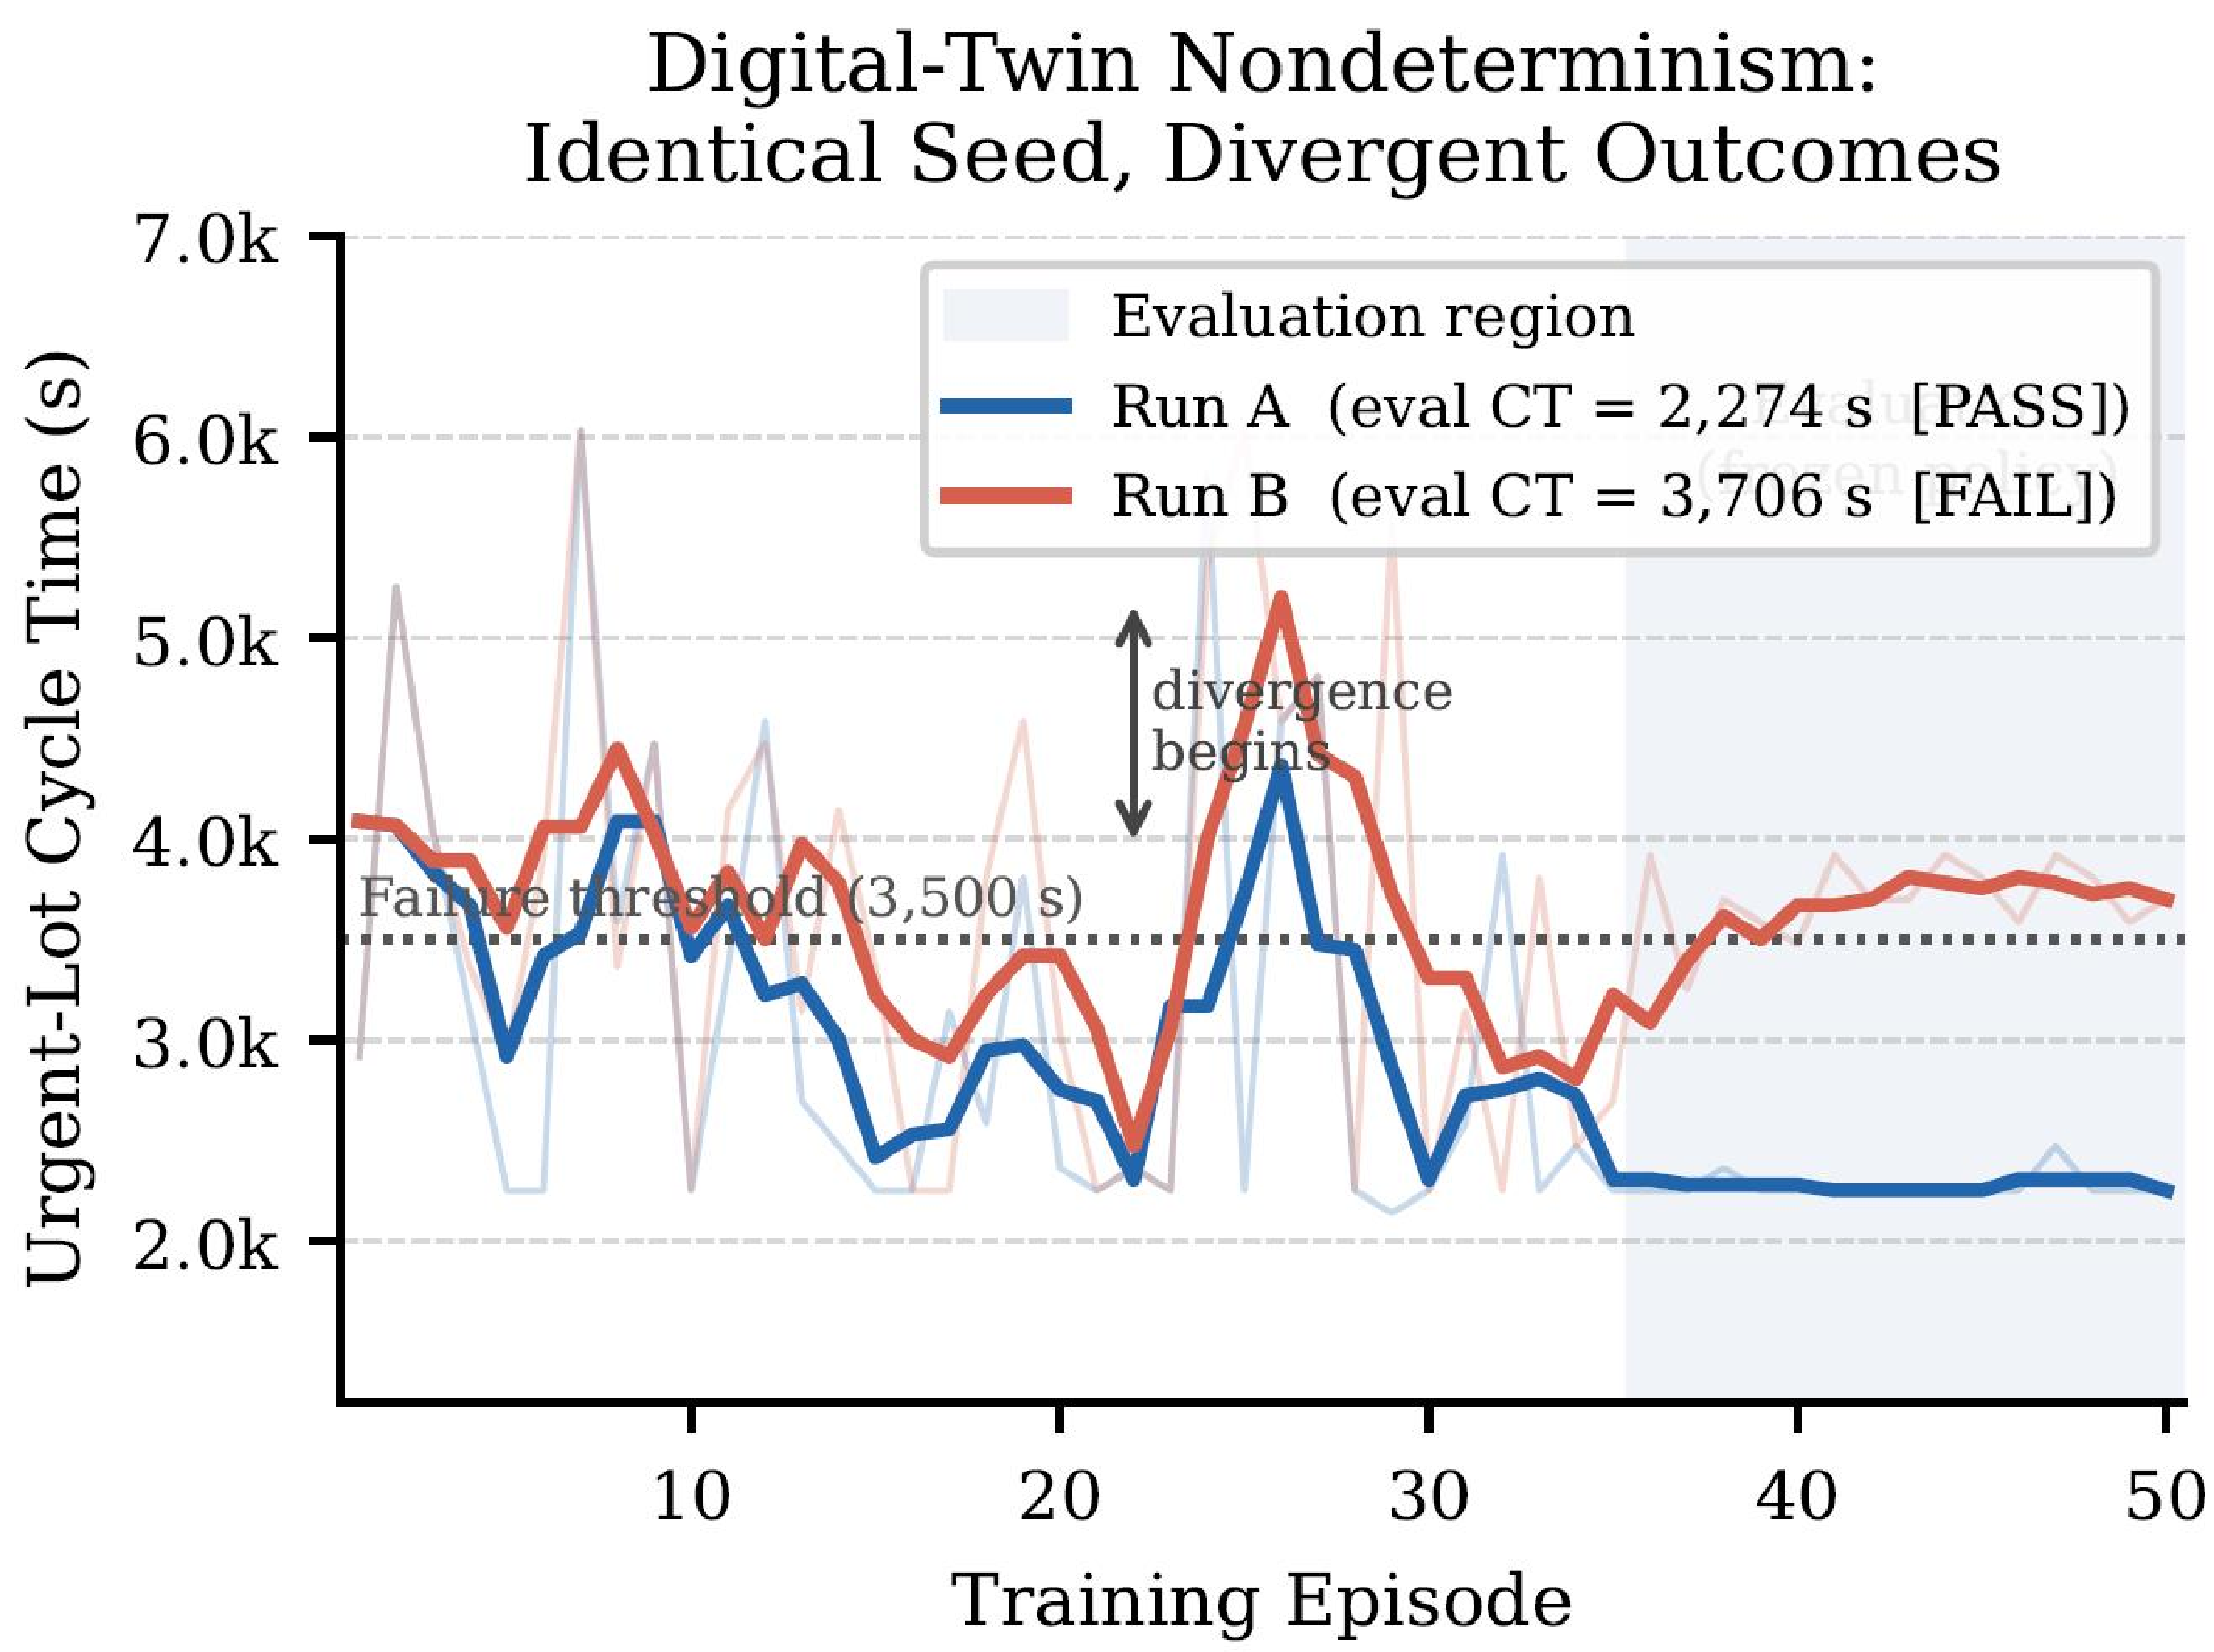
\includegraphics[width=0.98\columnwidth]{Figures/fig_nondeterminism.pdf}
  \caption{Digital-twin nondeterminism. Two pure-DRL runs with \emph{identical}
  random seed and configuration share a near-identical trajectory for
  $\sim$20 episodes, then diverge as simulator-level timing differences---invisible
  to the Python RNG---are amplified through learning: one converges to a passing
  policy, the other to a failing one. A fixed seed therefore does not reproduce an
  outcome, motivating distributional reporting over many seeds.}
  \label{fig:nondeterm}
\end{figure}

\paragraph{Reliability protocol.}
Because the digital twin is internally nondeterministic, a fixed seed does not
reproduce an outcome (Figure~\ref{fig:nondeterm}), so multiple independent seeds
are necessary. The causal chain is short but consequential: sub-RNG timing jitter
in the simulator yields slightly different state transitions, which enter the
replay buffer, perturb the fitted $Q$-values, and---compounded over training---can
tip the policy into a different basin of attraction, one passing and one failing
(the \emph{fault}$\rightarrow$\emph{error}$\rightarrow$\emph{failure} chain in
Laprie's taxonomy); our governance layer breaks this chain during training.
Following best practice for distributional reporting in RL
\citep{henderson2018,agarwal2021}, we run each condition for $N{=}20$ seeds and
report failure rates and variance, not single-run means. Each run executes 100
episodes; reward curves stabilize before episode 70
(Figure~\ref{fig:convergence}), so the final 30 episodes (71--100) capture
settled behavior, during which rules are frozen and the agent acts greedily.

\paragraph{Agent configuration.}
Rainbow DQN with hidden layers [1024, 512, 256], learning rate
$3\times10^{-4}$, discount $\gamma=0.98$, replay capacity 100k, multi-step
$n=3$, and target updates every 300 steps. Hyperparameters follow standard
Rainbow defaults \citep{hessel2018} and are held fixed across all conditions.

% ============================ 5. RESULTS ============================
\section{Main Results}
\label{sec:results}

\begin{figure}[t]
    \centering
    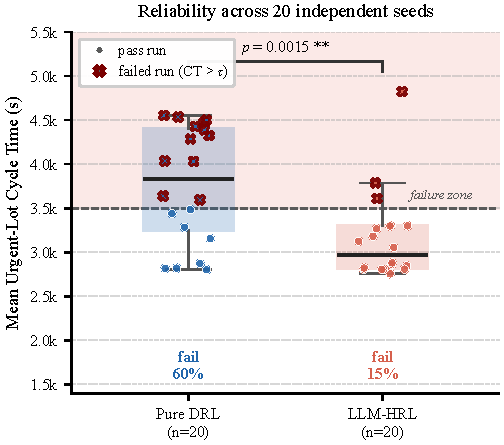
\includegraphics[width=0.86\columnwidth]{Figures/fig_reliability.pdf}
    \caption{Reliability across 20 independent seeds. Each marker is one run's
    mean evaluation CT; $\times$ marks runs in the catastrophic-failure zone
    ($\text{CT}>\tau$). Pure DRL fails in 60\% of runs, while LLM-HRL fails in
    15\%, with substantially lower spread ($p=0.0015$, two-sample $t$-test).}
    \label{fig:reliability}
\end{figure}

\paragraph{LLM-HRL is more reliable than pure DRL.}
Figure~\ref{fig:reliability} reports the central result. Pure DRL fails
catastrophically in 60\% of runs (12/20), whereas LLM-HRL fails in only 15\%
(3/20), a 45-percentage-point reduction. Mean CT drops from 3{,}773\,s to
3{,}148\,s ($-625$\,s, $-16.6\%$), and the spread tightens markedly (std
656\,s\,$\to$\,492\,s). The difference is significant and large: a two-sample
$t$-test on per-seed means gives $t=-3.41$, $p=0.0015$, Cohen's $d=1.08$, with a
95\% confidence interval on the CT reduction of $[253,997]$\,s; a bootstrap 95\%
CI on the failure-rate reduction is $[20,70]$ percentage points (Wilson intervals
on the failure rates themselves are $[39,78]\%$ for pure DRL and $[5,36]\%$ for
LLM-HRL). Production attainment is statistically unchanged across conditions
($p>0.05$), so governance removes the failure tail \emph{without} sacrificing
throughput.

\paragraph{The improvement is the removal of a failure mode.}
What changes is the failure cluster, not the average: rather than a uniform
speed-up, governance eliminates pure DRL's high-CT mode. The governed agent does not outperform a
\emph{lucky} DRL run---both reach similar cycle times---but it removes the
\emph{unlucky} runs, collapsing almost the entire outcome mass into the success
cluster. Figure~\ref{fig:convergence} shows the same effect during training: the
LLM-HRL mean tracks below pure DRL with a much narrower $\pm$1\,SD band, and
converges steadily below the failure threshold.

\begin{figure}[t]
    \centering
    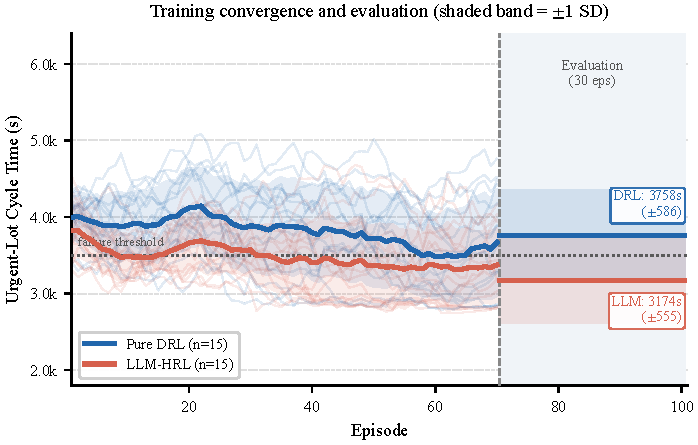
\includegraphics[width=0.98\columnwidth]{Figures/fig_convergence.pdf}
    \caption{Training convergence over 100 episodes (thin lines: individual
    seeds; bold: mean; shaded band $=\pm$1\,SD). The shaded region (episodes
    71--100) is the frozen-policy evaluation window, summarized by the horizontal
    mean lines and boxes. Pure DRL stays elevated and highly variable, settling
    above the failure threshold; LLM-HRL converges to a low, stable cycle time
    well below it. Both stabilize before episode~70, confirming the evaluation
    window captures settled behavior.}
    \label{fig:convergence}
\end{figure}

\paragraph{Sparse governance shapes the learned policy.}
A striking property is that during evaluation the frozen rules fire on fewer
than 2\% of steps, yet the governed agent is consistently dependable. This
indicates that the value of governance lies in \emph{when}, not \emph{how
often}, it intervenes: a handful of well-timed maskings during training---when an
urgent lot is present and the urgent-lot action should be taken---teach the agent
a behavior pure DRL acquires only by luck. Governance corrects the training
trajectory rather than filtering at runtime.

\subsection{Generalization across conflict regimes}
\label{sec:sweep}
Is the benefit specific to one operating point? To find out we
vary the urgent-lot density across three regimes---1.6\%, 4.7\%, and 7.7\% of all
lots---and measure both conditions (Figure~\ref{fig:sweep}). At low density
(1.6\%) urgent lots rarely contend for the bottleneck, and both methods succeed
with near-identical cycle time: governance is neither needed nor harmful. As
density rises, conflicts intensify and pure DRL begins to fail---reaching a 60\%
failure rate at both 4.7\% and 7.7\%---while LLM-HRL keeps the failure rate
strictly lower at every regime (0\%, 40\%, 15\%) and its cycle time below or near
$\tau$. The governance margin therefore \emph{grows with conflict density},
exactly where the resource stakes are highest. This identifies the regime in
which dependable governance delivers its impact and shows the effect is not an
artifact of a single configuration.

\begin{figure}[t]
    \centering
    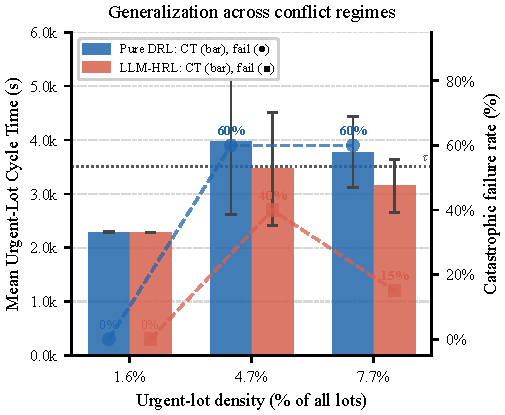
\includegraphics[width=0.92\columnwidth]{Figures/fig_sweep.pdf}
    \caption{Generalization across urgent-lot conflict regimes (bars: mean CT,
    $\pm$1\,SD; dashed: catastrophic failure rate). At low density both methods
    succeed; as conflicts intensify, pure DRL fails while LLM-HRL keeps the
    failure rate strictly lower at every regime. The governance benefit grows
    with conflict density.}
    \label{fig:sweep}
\end{figure}

% ============================ 6. ABLATION ============================
\section{Ablation: What Makes Governance Work?}
\label{sec:ablation}

The main result establishes \emph{that} LLM governance helps; this section
isolates \emph{why}. Our full method combines three properties: action
constraints that are \emph{hard} (mask, not reward), \emph{contextual}
(KPI-conditioned), and \emph{adaptive} (revised each episode). We test each by
removing exactly one property at a time, holding the reward function and the L0
agent fixed, and report five seeds per variant against the 20-seed full model and
pure-DRL anchors. Figure~\ref{fig:ablation} summarizes all conditions.

\begin{figure*}[t]
    \centering
    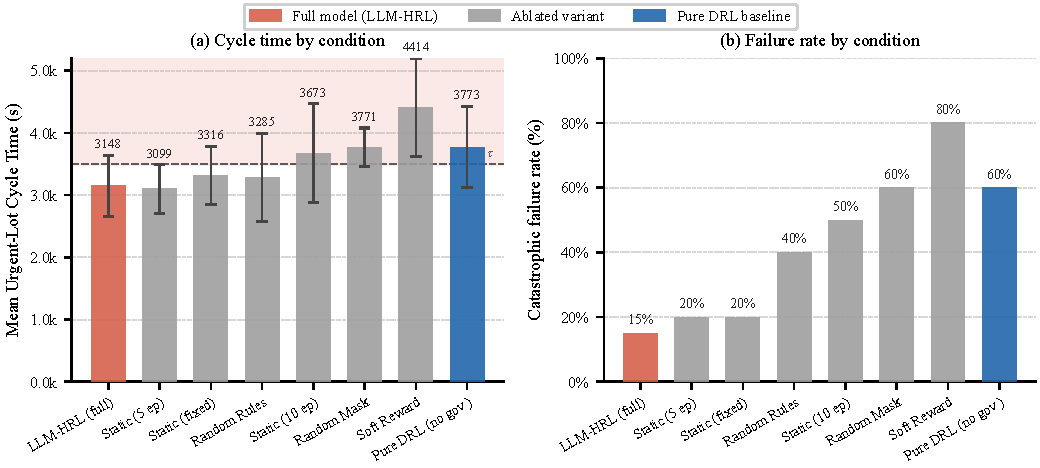
\includegraphics[width=0.92\textwidth]{Figures/fig_ablation.pdf}
    \caption{Single-axis ablation (mean of per-seed results; error bars
    $=\pm$1\,SD; ablated variants are a 5-seed pilot, full model and Pure DRL use 20).
    Each ablated variant removes exactly one property of the full model.
    \textbf{(a)} Mean cycle time; the shaded region is the failure zone
    ($\text{CT}>\tau$). \textbf{(b)} Catastrophic failure rate. Removing the hard
    mask (Soft Reward) is worse than ungoverned DRL; removing context (Random
    Mask) is no better than ungoverned DRL; and removing adaptivity (Rule-Based)
    matches the full model's average cycle time yet fails in 60\% of runs. Only
    the full model---hard, contextual, and adaptive---attains both low cycle time
    and a low failure rate.}
    \label{fig:ablation}
\end{figure*}

\paragraph{Removing hardness: mask $\to$ reward shaping.}
We replace the L1 action mask with an equivalent \emph{reward-shaping} term that
penalizes the same actions the mask would forbid, keeping the governance signal
identical but ``soft.'' This \emph{Soft Reward} variant is the worst condition we
test: mean CT rises to 4{,}414\,s with an 80\% failure rate---\emph{worse than
ungoverned pure DRL} (3{,}773\,s, 60\%) and significantly worse than our method
($p<0.001$). The reason is instructive: a shaping term large enough to dominate
at conflict time also distorts the far more frequent non-conflict periods,
injecting a non-stationary target that destabilizes learning. Hard masking
sidesteps this by pruning actions only when a rule fires, leaving the reward
undistorted. \emph{The benefit of governance is the hard constraint, not the
signal it encodes.}

\paragraph{Removing context: conditioned $\to$ random masking.}
We next ask whether \emph{any} action constraint suffices. The \emph{Random Mask}
variant applies masks of the same average frequency as LLM-HRL but at random
episodes and to random actions, ignoring KPIs entirely. It fails in 60\% of runs
(vs.\ 15\% for our method, $p<0.05$) with mean CT 3{,}771\,s---essentially
indistinguishable from ungoverned DRL. Constraining the action space helps only
when the constraint is applied \emph{in the right context}: masking the wrong
actions, or at the wrong time, confers no reliability benefit. \emph{When the
constraint fires matters as much as that one exists.}

\paragraph{Removing adaptivity: episodic $\to$ fixed rules.}
Finally we test the value of episodic revision with a \emph{Rule-Based} variant:
the same L1 enforcement and L0 agent as LLM-HRL, but driven by a fixed,
hand-crafted rule (forbid non-urgent actions when more than two urgent lots are
waiting) with no LLM revision. This is the most revealing comparison. On
\emph{average} it nearly matches our method (mean CT 3{,}347\,s vs.\ 3{,}148\,s;
the difference is not significant, $p=0.43$), which might suggest a fixed rule is
``good enough.'' Yet it still fails in 60\% of runs, and individual evaluation
episodes spike as high as 8{,}567\,s. A static rule constrains exploration even
in episodes where no urgent conflict arises, persistently distorting the policy
much as reward shaping does; it forecloses the lucky trajectories pure DRL can
still occasionally find, leaving structurally worse failures. \emph{Matching the
average is not the same as removing the tail---adaptation is what removes it.}

\paragraph{Summary.}
The single-axis ablation gives a clear verdict: each of the three
properties---hard, contextual, adaptive---is necessary, and removing any one
collapses reliability to the ungoverned 60--80\% failure regime. The full model
is the only condition that achieves both a low cycle time and a low failure rate
(Figure~\ref{fig:ablation}). Notably, the value of the LLM is precisely that it
supplies all three properties at once, automatically and without hand
engineering, while attaching a human-readable rationale to every rule.

% ============================ 7. DISCUSSION ============================
\section{Discussion}
\label{sec:discussion}

Our results reframe what LLM-over-DRL governance is \emph{for}. The governed
agent does not beat a lucky pure-DRL run; its value is eliminating the unlucky
runs---the catastrophic schedules that arise intermittently from digital-twin
nondeterminism. In manufacturing, where one badly scheduled urgent lot can
cascade into quality-time violations and yield loss, removing the failure tail is
worth more than a marginal average improvement. This aligns the contribution with
dependability engineering \citep{avizienis2004}: the \emph{fault} is
unobservable simulator nondeterminism; the \emph{error} is a policy that
under-prioritizes urgent lots when the fault corrupts training; and the
\emph{failure} is $\overline{\mathrm{CT}}>\tau$. Governance is a
\emph{fault-tolerance mechanism}: it breaks the fault$\to$error$\to$failure chain
by steering the policy during training, much as redundancy does in classical
fault-tolerant systems.

The ablation sharpens this into an actionable design principle: the benefit is
\emph{not} the LLM per se, nor the injection of any external signal, but the
\emph{hard, contextual, and adaptive} pruning of unsafe actions. The overhead of
delivering it is negligible: one LLM call per episode ($\approx$2--5\,s), 2--4
rules, and microsecond-scale L1 evaluation per step.

\paragraph{Why an LLM, and not hand-crafted rules?}
Since the operative ingredient is hard, contextual, adaptive masking, why not
hand-write the rules? The Rule-Based result answers: a fixed expert rule cannot
\emph{adapt} as the conflict pattern shifts and fails in 60\% of cases, while
recovering adaptivity by hand demands re-engineering the rule set for every
conflict regime and product mix---the brittle manual effort rule-based dispatch
is known for. Non-LLM \emph{adaptive} generators (online decision trees,
threshold optimizers, Bayesian rule updaters) could in principle supply the same
adaptivity, but typically need a hand-designed feature space, must be re-tuned per
line, and emit opaque parameters; the LLM instead yields adaptive, contextual,
\emph{auditable} rules zero-shot from natural-language knowledge, run locally
without exposing production data. A direct comparison remains future work.

\paragraph{Beyond manufacturing.}
Nothing in the framework is specific to semiconductors. The conditions that make
it valuable---a stochastic environment that induces run-to-run policy
unreliability, together with rare but costly events whose mishandling matters far
more than average throughput---recur in traffic-signal control, warehouse and
job-shop scheduling, cloud resource allocation, and emergency dispatch. In each,
an LLM that reads task-level KPIs and emits hard, contextual, auditable
constraints could harden an existing DRL controller without retraining. We
therefore view the contribution as a general recipe for dependable RL, with
semiconductor scheduling as a demanding instantiation rather than its boundary.

\paragraph{Deployment and resource implications.}
The approach is practical to deploy: it adds dependability to an existing agent
without retraining, runs locally on commodity hardware so that no production data
leaves the fab, and exposes every decision in language an operator can inspect
and override. In a resource-critical fab there is a further benefit---the
catastrophic tail is where Q-time violations, scrap, and rework concentrate, so
removing it also conserves the energy, water, and materials embodied in at-risk
lots. Improved reliability thus carries a direct resource-efficiency payoff
alongside the operational one.

% ============================ 8. LIMITATIONS ============================
\section{Limitations}
\label{sec:limitations}

All experiments are in simulation; live deployment would require real-time
equipment interfaces and formal safety qualification, and generalization across
products and fabs will require re-calibrating the digital twin. The ablation
variants use five seeds each, so we report their per-seed-mean differences
alongside failure rates and worst-case episodes rather than $t$-tests alone. Most
importantly, we do not compare the LLM against \emph{adaptive non-LLM} rule
generators (e.g., online decision trees or threshold optimizers); quantifying
whether they can match its zero-shot, auditable rules is the key next experiment.
Finally, on one seed a train/evaluation distribution shift left the final rule
inert, reducing that run to pure DRL; a stronger model or distribution-robust
thresholds may help.

% ============================ 9. CONCLUSION ============================
\section{Conclusion}

We treated an LLM not as a policy generator but as an adaptive governance module
that hardens an off-the-shelf DRL agent against catastrophic,
nondeterminism-induced failure. On urgent-lot scheduling in a semiconductor
digital twin built from real factory data, it cuts the catastrophic-failure rate
from 60\% to 15\% and mean cycle time by 625\,s ($p<0.01$, $N{=}20$ seeds)
without harming throughput, consistently across conflict regimes. A single-axis
ablation localizes the gain to \emph{hard, contextual, and adaptive} action
constraints: reward shaping is worse than no governance ($p<0.001$),
unconditioned masking is no better, and a fixed rule matches the average yet
leaves the failure tail intact. Beyond the resource savings this yields in a
fab---less scrapped material---we argue the broader contribution is to reframe
LLM-over-DRL governance as a general, local, and auditable mechanism for
\emph{dependable} reinforcement learning.

\bibliography{references}

\end{document}
